\chapter{Introduction}

This thesis will investigate and characterise an Indigenous seasonal calendar.
I combine Indigenous knowledge with Western climate science to characterise
local seasonality in NE Arnhem Land (see \autoref{fig:arnhem-map}),
as described by a Yolngu seasonal calendar I construct based on
interviews and supported by literature.\\

Previous research has focussed on the social or ecological aspects of Australian
Indigenous calendars.  This thesis instead treats Indigenous knowledge as a
\emph{framework for} research, not simply an \emph{object of} research.
Togther with an cross-disciplinary approach quantifying Indigenous seasons,
my results are highly novel -- and indeed, to my knowledge unique.



\section{About Indigenous Seasons}

Seasonal calendars are constructed by humans as a usefully simplified
abstraction of annual variation in the environment - whether physical
changes such as temperature, or social events from birthdays to financial
reporting.  The definitions of seasons carry knowledge about annual cycles,
and also the domain for which the calendar is applied - eg. temperature
or taxation.
%
Documenting and quantifying seasons defined by biophysical conditions
or events allows researchers to draw on a significant body of existing,
implicit, knowledge about the environment.
%
This knowledge supports decisions in a range of areas; from natural
resource management, agriculture, or energy demand forecasts, to
the timing of meetings and holidays or the materials used in high fashion.
Seasons have a profound impact on human societies, and understanding
them matters.\\


Australia formally recognises four seasons, defined by Gregorian date:
Summer begins on December 1\textsuperscript{st}, Autumn on March
1\textsuperscript{st}, Winter on June 1\textsuperscript{st}, and Spring
on September 1\textsuperscript{st} \citep{wells2013}. This follows the
meteorological standard for seasons, originating in Europe (REF), rather
than the solar seasonal calendar marked by solsticies and equinoxes.
%
Throughout the temperate zone, seasons are informally recognised more by
temperature than date (Summer being the hottest and Winter the coldest time
of year), and thus varying from year to year.  While rainfall is often
strongly  seasonal the relationship varies from place to place, and it is
less recognised as an indicator.
%
However, temperate seasons are essentially irrelevant to the tropical and
equatorial climate of northern Australia.  In these areas a monsoonal Wet
and Dry season dominate, generally recognised by weather conditions.
This system is highly simplistic, lacking any of the nuance or local
knowledge embedded in Indigenous calendars.  Australia can, and should,
do better.\\


Australian Indigenous seasons are defined by weather and ecological events.
They are typically recognised after the fact, and vary in timing and length
between years depending on the behaviour of their indicators.  This study
focusses on the seasonal calendar of the Yolngu people, in Arnhem Land (see
\autoref{fig:arnhem-map}).
%
The Yolngu seasonal calendar is reasonably complex - see
\autoref{subsec:three-seasons-scales} - but there are six major seasons
analysed below, defined by prevailing wind, rainfall, temperature, and a
variety of other factors.  The exact definitions are highly localised,
and vary slightly even between communities sharing the same language.




\section{Contribution of this Research}
\label{sec:intro-contribution}

\textit{
Needs to lay out the wider -- global -- story of why seasons are important,
which becomes a narrative thread throughout the thesis.
This should answer the `why bother' question, and justify the research.
Another ongoing thread is `multiple approaches yield richer results'.
%
Paragraph on the global-scale reason to care about the topic.
Explain and compare to phenology and ecological seasons.
Draw link from IK to IEK to ecological knowledge.
Explain shortcomings in existing research.
}
~\\



Links IEK to seasons.  Cover phenology as seasonal definer.
Explains (briefly; more in lit review!) the nature of previous research
and lack of quantification.  Go over how to quantify, and why
this is interesting.


See \citet{menzel2006} re modern scientific use of ecological changes
as indicators of seasonal onset or climate change.


Indigenous knowledge is recognised and valued in an increasing variety
of contexts \citep[eg.][]{petheram2010,cochran2015,berkes2012} –
but integration with the physical sciences is still relatively rare and ad-hoc.
%
I argue that such synthesis provides a crucial long-term perspective on
anthropogenic environmental change, and demonstrate that such synthesis
can produce novel results for both scientific and indigenous stakeholders.

Ecological knowledge is embedded in calendars.




\section{Research Context}
\label{sec:context}

This study focusses on North-East Arnhem Land, particularly Elcho Island
and the town of Galiwinku.  Figure~\ref{fig:arnhem-map} shows the study
area, on the north-east coast of the Northern Territory about five hundred
kilometers east of Darwin.
%
These sites fall within the Anrhem Coast bioregion \citep{ens2014}.
The landscape is dominated by tropical woodland, from mangroves on the coastline
through dense forest to more open woody grasslands further inland.
%
Qualitative seasonality is described for Galiwinku and Milingimbi;
quantitative weather observations are from Waruwi, Maningrida, Milingimbi,
Galiwinku, and Nhulunbuy.  Waruwi and Maningrida are in areas described by
other calendars, but provide a longer weather record in a similar climate.

\begin{figure}[h]
    \centering
    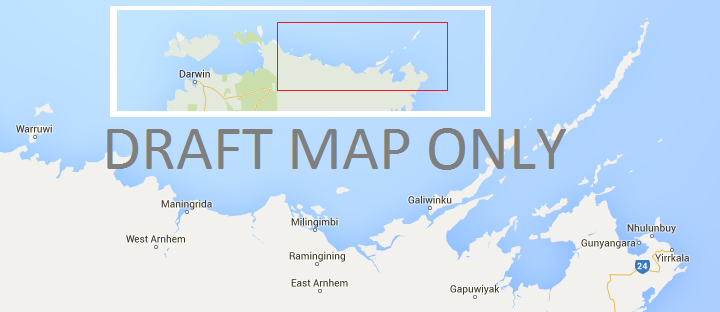
\includegraphics[width=\textwidth]{mapdraft.png}
    \caption[Map showing the study area, NE Arnhem Land]{
        Map showing the study area, NE Arnhem Land.
        Analysis in \autoref{ch:quantify} uses weather observations from several of the towns shown.
        TODO:  better map (inset all Aus), label towns and referenced place names
        (Elcho Island, etc.)
        Would also be good to shade by Indigenous group, approximately.
        }
    \label{fig:arnhem-map}
\end{figure}

The Yolngu calendar and this study area were chosen as the case study for
this thesis for several reasons.  Personal connections and logistical support
from the Uniting Church greatly facilitated qualitative research.  The
Yolngu seasons emphasise meteorological indicators, which allows principled
quantification based on the observational weather record.  Finally, research
on Indigenous seasons or even nuanced tropical seasons is rare in Australia,
and may be valuable in informing traditional or western land and natural
resource management.

In a letter inviting collaboration on this research (see \autoref{sec:ethics}),
a senior Yonlgu man explained that \blockquote{
    For Yolngu (the people of North Eastern Arnhem Land) it is the Liyagadhaman
    who carry within them the wisdom and knowledge of these matters.
    It is right that in this research you have approached me to talk about these
    things. I can also introduce you to others who have this knowledge.  ...

    Yolngu have made careful observation of the ways of nature and the seasons
    over the millennia and have passed on that knowledge down the generations.
    We know the changes that are taking place in the seasons and I am willing
    to talk with you about what I have seen happening around me.
}

\citet{woodward2012b} explains four key aspects of Indigenous seasonal
knowledge systems: \blockquote{
    a focus on resource use, knowledge of complex ecological indicators
    to facilitate resource collection, knowledge of meteorological
    phenomena and a strong metaphysical/spiritual understanding.}.
This emphasises the nuance and value of Indigenous knowledge of tropical
seasonality, which goes far beyond the Wet/Dry/Buildup cycle recognised
by non-Indigenous locals \citep{willmett2009}.

The key meteorological determinants of seasonality are temperature (especially
night-time), rainfall, humidity, and wind strength and direction; the annual
cycle is driven primarily by the Indian Ocean monsoon.  The climate is hot and
humid, with daytime temperatures between 25 and 40 degrees year-round.



\section{Thesis Structure}

The chapters of this thesis -- Introduction, Literature Review, Methods,
Results, Discussion, and Conclusion -- follow the usual convention for
a scientific report.  Within the Methods and Results chapters
the structure is slightly more complicated, due to the use of iterative and
cross-disciplinary approaches.  Quantitative methods are informed by
qualitative results, necessitating forward references.  Readers may wish
to read these chapters as paired sections, which reflects the research
process.\\


The introduction (this chapter) briefly introduces the topic of
indigenous seasons, the contribution of this research, context and
study area, and outlines the structure and scope of the thesis.
%
\nameref{ch:lit-review} (\autoref{ch:lit-review}) reviews prior research
on indigenous seasons and relevant methods.  Note that other chapters
also reference literature where relevant.
%
\nameref{ch:methods} (\autoref{ch:methods}) lays out the methods used in
qualitative research with Indigenous participants, quantitative meteorological
descriptions, and the methodological approach to synthesis.

\nameref{ch:results} (\autoref{ch:results}) presents qualitative and
quantitative results, including interpretation of figures.
%
\nameref{ch:discussion} (\autoref{ch:discussion}) interprets and discusses
all results.  It also reflects on methods used and created, novelty and
potential applications, and directions for further study.
%
\nameref{ch:conclusion} (\autoref{ch:conclusion}) summarises the findings
and impact of the research.

The appendicies (see \autoref{ch:appendicies}) are split into two parts.
The printed appendicies are included with this document, and contain
important data such as additional figures or details of the human ethics
approval which would be disruptive in the main text.  The second part
is the electronic appendicies, which contains all other material judged to
be useful for further study - including all numerical data and scripts
needed to reproduce the results.



\section{Scoping and Delimitations}
Indigenous Knowledge is a fascinating field, and would bear substantially
more study than is possible within the time and resource constraints of
an Honours thesis.

This research investigates Yolngu seasons in North-East Arnhem Land, in
the area of Galiwinku and Milingimby.  The qualitative data describes the
definitions of seasons and conditions in recent decades; the quantitative
weather record begins with the installation of automatic weather stations
at several airports between 1990 and 2003.  The results do not support
speculatation on the past or future state of Yolngu seasons.  The methods
however are applicable to data such as cliamte models, which provide
a clear direction for further work.

The research questions are:
\begin{itemize}
\item How are Yolngu seasonal calendars defined, and does this vary?
\item Which Yolngu calendar is best suited for mixed-methods study?
\item What are the properties and changes that define this calendar?
\item How may these seasons be characterised by meterological parameters?
\end{itemize}
These questions follow the same four-step methodology as the project itself:
understand the system to ask meaningful questions; identify key
qualitative information; apply insights to construct exact definitions; and
finally conduct quantative analysis.


This research is not a deep or rigorous exploration of historical Yolngu
perspectives; all interviews were conducted in English and in Darwin, and
the small number of participants limits investigation of the social or
cultural aspects of Indigenous Knowledge.  The climatological analysis
does not consider trend change, or more than basic correlation with
wider climatic forcings.
%
Instead, the novelty and value of this work is in synthesis: bringing
togther Yolngu perspectives on the natural environment, and the
data-oriented approach of climate science.  No prior work of this kind
could be identified in the literature.  The results have potential to
teach both scientists and Yolngu people about alternative perspectives,
and to appreciate their value.

